\chapter{\uppercase{Neutrinos}} \label{ch:Neutrinos}

\section{Discovery of the Neutrino} \label{sec:NeutrinoDiscovery}

The study of radioactive decay in the early 20th century exposed discrepancies that would lead to the postulation and eventual discovery of the neutrino.
An experiment performed by Lise Meitner and Otto Hahn in 1911 offered some of the first evidence that the energy spectrum of electrons emitted by beta decay is continuous \cite{Hahn:1911}. 
This was in stark contrast to the expected discrete spectra that had been observed in gamma and alpha emission, and suggested that three laws of conservation (energy, linear momentum, and angular momentum) were broken during beta decay. 
Their findings were later confirmed by experiments performed by Chadwick in 1914 \cite{Chadwick:1914zz} and Ellis and Wooster in 1927 \cite{Ellis:1927}. 

At the time, beta decay was thought to be a two-particle decay, a process that yields a product nucleus and an electron.
In 1930, Wolfgang Pauli postulated a particle he called the `neutron', which would be ejected with the electron, thereby conserving energy and momentum.
Describing his idea as a ``desperate remedy'', this new particle would have to be neutral and non-interacting, therefore making it almost impossible to detect.
In 1934, Enrico Fermi further developed the theory of beta decay, including Pauli's particle but renaming it the neutrino, meaning ``little neutral one'' \cite{Fermi:1934hr}.
Due to the nature of the weakly interacting neutrino, experimental discovery would take another 20 years.

In 1956 Clyde Cowan and Fred Reines accomplished the amazing feat of discovering this elusive particle experimentally by taking advantage of the inverse beta decay (IBD) process \cite{Cowan}:

\begin{equation}
	\bar{\nu} + p \rightarrow n + e^{+}
\end{equation}

Their idea was to place a detector near an intense source of neutrinos, fill it with an ample number of protons, and observe the resulting positrons. 
However, any source that generates a large enough flux of neutrinos will create large backgrounds for the experiment. 
As would become the challenge for every neutrino detector thereafter, Cowan and Reines had to devise a way to reduce the background such that they could obtain a measurable and believable number of neutrinos.
Their original idea was to place a detector underground about 40 meters away from a fission bomb. 
This would create a large instantaneous flux of neutrinos providing a sufficient signal to background ratio. 

After some thought, though, they realized that by detecting the neutron \textit{and} the positron they could discriminate the IBD signal from the background with much higher success. 
This would allow the use of a nuclear reactor instead of a fission bomb as a neutrino source, giving them the opportunity to patiently watch for neutrinos rather than be restricted to one chance with a bomb. 
The final detector that would facilitate the discovery of the electron anti-neutrino, $\bar{\nu_{e}}$, contained 1400 liters of liquid scintillator viewed by 110 photomultiplier tubes and 200 liters of water with dissolved cadmium chloride, and was placed near the fission reactor at the Savannah River Plant in South Carolina. 

The mechanisms behind the detector developed by Cowan and Reines worked as follows. 
Neutrinos from the reactor enter the detector and interact with protons in the water. 
The positron resulting from this reaction quickly collides with an electron, creating two gamma rays which Compton scatter and initiate a cascade of electrons that causes the liquid to scintillate. 
Simultaneously, the neutron from the initial reaction bounces around as it collides with protons until, eventually, it captures on a cadmium nucleus and releases about a 9 MeV gamma ray, also causing the liquid to scintillate. 
The time between the flash of light from the positron annihilation and that of the neutron capture is on the order of microseconds. 
It was by looking for this delayed-coincidence signature that Cowan and Reines were able to successfully detect the first neutrino, and thus pave the way for future neutrino experiments. 

Only 6 years after the discovery by Cowan and Reines, Lederman, Schwartz, and Steinberger discovered the muon neutrino, $\nu_{\mu}$ \cite{Lederman},
but the discovery of the tau neutrino, $\nu_{\tau}$, by the DONUT (Direct Observation of the Nu Tau) experiment would not occur until 44 years later \cite{TauDONUT,DONUT}.


\section{Neutrinos in the Standard Model and Beyond} \label{ch:NeutrinosInSM}

The Standard Model (SM) of particle physics is the result of several decades of work by many scientists. It is a field theory that describes three of the four fundamental forces (electromagnetic, strong and weak), and classifies all known elementary particles as outlined in Table~\ref{tab:SM}.

%It is invariant under SU(2)$_L \times$ U(1) transformations, where the subscript $L$ indicates that the SU(2) transformation operates on the left-handed chiral components of the fields.

\begin{table}
	\centering
\begin{tabular}{|c|c|c|c|c|c|c|}
	\hline 
	& \multicolumn{3}{c|}{\textbf{Fermions}} & & \multicolumn{2}{c|}{\textbf{Bosons}}  \\ 
	& \multicolumn{3}{c|}{spin = 1/2} & & spin = 1 & spin = 0 \\
	\hline 
	Generation & I & II & III & & Gauge Bosons & Scalar Bosons \\ 
	\hline 
	Quarks & u & c & t & & g & H \\ 
	%\hline 
	& d & s & b & & $\gamma$ &  \\ 
	%\hline 
	Leptons & e & $\mu$ & $\tau$ & &  Z &  \\ 
	%\hline 
	& $\nu_{e}$ & $\nu_{\mu}$ & $\nu_{\tau}$ & & W &  \\ 
	\hline 
\end{tabular}
\caption[The Standed Model of Particle Physics]{The Standard Model of particle physics, composed of fermions and their corresponding antiparticles, the force carries (gauge bosons), and the Higgs boson.}
\label{tab:SM}
\end{table}

Classified in three generations of leptons, neutrinos exist in corresponding flavors, electron neutrinos ($\nu_{e}$), muon neutrinos ($\nu_{\mu}$), and tau neutrinos ($\nu_{\tau}$), to the electron (e), muon ($\mu$), and tau ($\tau$) leptons, respectively.
For each of these flavors a corresponding antiparticle also exists, $\bar{\nu_e}, \bar{\nu_\mu}, \bar{\nu_\tau}$.

If neutrinos have exactly zero mass and travel at the speed of light, then by definition their helicity, or handedness, is a conserved property. 
Since experiments only measured left-handed neutrinos \cite{PhysRev.109.1015}, it was assumed that all neutrinos in the SM were massless.
As will be discussed in greater depth in Section~\ref{sec:NeutrinoOsc}, it was later experimentally discovered that neutrinos oscillate, or change flavors, indicating that at least two of the three neutrinos must have mass.

Their ability to oscillate arises from the fact that neutrinos exist as flavor eigenstates of the weak interaction, $\nu_\alpha$: $\alpha = e, \mu, \tau$, that are not identical to their mass states, $\nu_i$: $i = 1, 2, 3$, which are eigenstates of the Hamilton describing the free neutrino.
This means that a neutrino produced at a source has a known flavor, but its mass is described as a superposition of all possible mass eigenstates, creating three possible scenarios:
(i) The mass states are the same as the flavor states, therefore, a neutrino produced as a $\nu_x$ will remain $\nu_x$ forever. 
(ii) The mass states and flavor states are different, but the mass states are all the same or all zero, therefore, a neutrino produced as $\nu_x$ will still remain $\nu_x$ because the combination of mass states does not change over time. 
(iii) The mass states and flavor states are different and at least two of the mass states are not the same, therefore, the phase between mass states will change as the neutrino propagates through time and space causing a change of flavor state.
Experimental discoveries of neutrino oscillation require that the third scenario is correct.

Given this we can define the probability that a neutrino oscillates by first describing the flavor eigenstates as:
\begin{equation}
	\ket{\nu_\alpha} = \sum_{i}U_{\alpha i}\ket{\nu_i}
\end{equation}
where U$_{\alpha i}$ is the unitary Pontecorvo-Maki-Nakagawa-Sakata (PMNS) mixing matrix \cite{PDG}. 
The PMNS matrix relates flavor to mass eigenstates and can be written in factorized form as:
\begin{equation}	
	U = 
	\begin{pmatrix}
		1 & & \\
		& c_{23} & s_{23} \\
		& -s_{23} & c_{23}
	\end{pmatrix}
	\begin{pmatrix}
		c_{13} & & s_{13}e^{-i\delta} \\
		& 1 &	\\
		-s_{13}e^{i\delta} & & c_{13}
	\end{pmatrix}
	\begin{pmatrix}
		c_{12} & s_{12} & \\
		-s_{12} & c_{12} & \\
		& & 1
	\end{pmatrix}
	\begin{pmatrix}
		1 & & \\
		& e^{i\alpha}  & \\
		& & e^{i\beta}
	\end{pmatrix}
\end{equation}
where $s_{ij} = \sin\theta_{ij}$ and $c_{ij} = \cos\theta_{ij}$, $\theta_{ij} = [0,\pi/2]$,
$\delta = [0,2\pi]$ is the Dirac charge parity (CP) violation phase, and $\alpha$ and $\beta$ are two Majorana CP violation phases.

As a neutrino, $\nu_\alpha$, propagates in time the mass eigenstates evolve differently (assuming that $m_{1} \neq m_{2} \neq m_{3}$), resulting in a new flavor state, $\nu_{\beta}$.
Massive neutrinos move through time and space as
\begin{equation}
	\ket{\nu_i(x,t)} = e^{-\frac{i}{\hbar}(E_{i}t-\vec{p}_{i}\cdot\vec{x})}\ket{\nu_i(0,0)} = e^{-i\phi}\ket{\nu_i(0,0)} 
\end{equation}
The flavor state $\alpha$ at some point in time and space can then be defined as:
\begin{equation}
	\ket{\nu_{\alpha}(x,t)} = \sum_{i}U_{\alpha i}\ket{\nu_{i}(x,t)} = \sum_{i}U_{\alpha i}e^{-i\phi_{i}}\ket{\nu_{i}(0,0)}
\end{equation}
Therefore, the oscillation probability that a neutrino produced as flavor $\nu_\alpha$ will be detected as flavor $\nu_\beta$ after traveling for a period of time is given by 
\begin{equation}	
\begin{split}
	P(\nu_\alpha \rightarrow \nu_\beta) &= \abs{\bra{\nu_\alpha(0,0)}\ket{\nu_\beta(x,t)}}^2 \\
	%&=\abs{\sum_i U^{*}_{\alpha i} \sum_{j}U_{\beta j}e^{-i\phi_j}\bra{\nu_i(0,0)}\ket{\nu_j(0,0)}}^2 \\
	%&=\abs{\sum_{i}\sum_{j}U^{*}_{\alpha i}e^{-i\phi_j}U_{\beta j}\delta_{ij}}^2 \\
	&=\abs{\sum_{i}U^{*}_{\alpha i}e^{-i\phi_i}U_{\beta i}}^2 \\
	%&=\sum_{i}U^{*}_{\alpha i}e^{-i\phi_i}U_{\beta i} \sum_{k}U_{\alpha k}e^{i\phi_k}U^{*}_{\beta k} \\
	&=\sum_{i}\sum_{k}U^{*}_{\alpha i}U_{\beta i}U_{\alpha k}U^{*}_{\beta k}e^{-i(\phi_{i}-\phi_{k})}
\end{split}
\end{equation}

This is true for any number of neutrino generations, but for the sake of simplicity, consider the case of two neutrino oscillation. In this scenario the mixing matrix can be written as 
\begin{equation}	
U = 
\begin{pmatrix}
U_{\alpha 1} & U_{\alpha 2} \\
U_{\beta 1} & U_{\beta 2}
\end{pmatrix} = 
\begin{pmatrix}
\cos\theta_{12} & \sin\theta_{12} \\
-\sin\theta_{12} & \cos\theta_{12}
\end{pmatrix}
\end{equation}
Therefore, the probability of oscillation is given by
\begin{equation}
\begin{split}
P^{2\nu}(\nu_\alpha \rightarrow \nu_\beta) 
%&= \sum_{i=1,2}\sum_{k=1,2}U^{*}_{\alpha i}U_{\beta i}U_{\alpha k}U^{*}_{\beta k}e^{-i(\phi_{i}-\phi_{k})} \\
%&= \abs{U_{\alpha 1}}^{2}\abs{U_{\beta 1}}^2 + 
%U^{*}_{\alpha 1}U_{\beta 1}U_{\alpha 2}U^{*}_{\beta 2}e^{-i(E_1-E_2)} + 
%U^{*}_{\alpha 2}U_{\beta 2}U_{\alpha 1}U^{*}_{\beta 1}e^{-i(E_2 - E_1)} +
%\abs{U_{\alpha 2}}^2\abs{U_{\beta 2}}^2 \\
&=  \abs{U_{\alpha 1}}^{2}\abs{U_{\beta 1}}^2 + \abs{U_{\alpha 2}}^2\abs{U_{\beta 2}}^2 +
U^{*}_{\alpha 1}U_{\beta 1}U_{\alpha 2}U^{*}_{\beta 2}(e^{i(\phi_2-\phi_1)} + e^{-i(\phi_2 - \phi_1)}) \\ 
%&= \cos^2\theta \sin^2\theta  + \sin^2\theta\cos^2\theta - 2\cos\theta \sin\theta \sin\theta \cos\theta \cos(E_2-E_1) \\
%&= 2\cos^2\theta\sin^2\theta -2\cos^2\theta\sin^2\theta\cos(E_2-E_1)\\
%&= 2\cos^2\theta\sin^2\theta(1-cos(E_2-E_1)) \\
%&= 2\cos^2\theta\sin^2\theta(2\sin^2(\frac{E_2-E_1}{2})) \\
%&= 2(\frac{1}{2}\sin{2\theta})^2(2\sin^2(\frac{E_2-E_1}{2})) \\
&= \sin^22\theta_{12}\sin^2\left(\frac{\phi_2-\phi_1}{2}\right)
\end{split}
\end{equation}
Now, recall that 
\begin{equation}
	\phi_i = \frac{1}{\hbar}(E_{i}t - \vec{p}_{i}\cdot\vec{x})
\end{equation}
The mass of the neutrino is very small compared to its energy ($m_\nu << E_\nu$) so 
the momentum can be approximated as
\begin{equation}
	p_i = \frac{1}{c}\sqrt{E^2_i-m^2_ic^4 } = \frac{1}{c}\left(E_i - \frac{m^2_ic^4}{2E_i} \right)
\end{equation}
If it is reasonably assumed that neutrinos move at the speed of light, $c$, then
the phase difference, $\phi_2 - \phi_1$, can be approximated as
\begin{equation}
\begin{split}
	\phi_2 - \phi_1 &= \frac{1}{\hbar}\left( (E_2 - E_1)\frac{L}{c} - (p_2 - p_1)L  \right)\\
	%&= \frac{1}{\hbar}\left( (E_2 - E_1)\frac{L}{c} - \left(E_2 - \frac{m_2^2c^4}{2E_2} - E_1 + \frac{m_1^2c^4}{2E_1}\right)\frac{L}{c}\right) \\
	%&=\frac{1}{\hbar}\frac{L}{c}\left(E_2 - E_1 - E_2 + \frac{m_2^2c^4}{2E_2} + E_1 - \frac{m_1^2c^4}{2E_1} \right) \\
	&=\frac{1}{\hbar}\frac{L}{c}\left(\frac{m_2^2c^4}{2E_2} - \frac{m_1^2c^4}{2E_1}\right) \\
	%&=\frac{1}{\hbar}\frac{L}{c}\frac{c^4}{2}\left(\frac{m_2^2}{E_2}-\frac{m_1^2}{E_1}\right) \\
	&=\frac{L}{\hbar c}\frac{\Delta m^2_{21}c^4}{2E}
\end{split}
\end{equation}
where $t = \frac{L}{c}$, $\Delta m^2_{21} = m_2^2 - m_1^2$ and $E_1 = E_2 = E$.

It can now be shown that the oscillation probability of a neutrino $\nu_\alpha$, being detected as flavor $\nu_\beta$ in the two neutrino mixing case is
\begin{equation}
	P^{2\nu}(\nu_\alpha \rightarrow \nu_\beta) = \sin^2\left(2\theta_{12}\right)\sin^2\left(\frac{c^4}{4\hbar c}\frac{\Delta m^2_{12}L}{E}\right) 
\end{equation}
The corresponding survival probability, the chance that a neutrino $\nu_\alpha$ is detected as $\nu_\alpha$, can be described by $P^{2\nu}(\nu_\alpha \rightarrow \nu_\alpha) = 1 - P^{2\nu}(\nu_\alpha \rightarrow \nu_\beta)$.

There are several aspects of note about this probability. It can be seen that the amplitude of the oscillation probability, $\sin^2\left(2\theta_{12}\right)$, depends on the mixing angle $\theta_{12}$, while the mass splitting, $\Delta m^2_{12}$, the energy of the neutrino, $E$, and the distance traveled, $L$, determine the frequency of oscillation. 
The probability is non-zero only when $\Delta m^2_{12}$ is non-zero, indicating that if an experiment observes neutrino oscillation, then at least one of the neutrinos must have mass.
Finally, the dependence of oscillation on the factor $\frac{L}{E}$ allows experiments to decide the placement of neutrino detectors based on what features of neutrinos they would like to study. 
Theoretical models alone do not prove neutrino oscillation, however. The first experimental evidence for oscillation and neutrino mass will be described in Section~\ref{sec:NeutrinoOsc}.

\section{Discovery of Neutrino Oscillation} \label{sec:NeutrinoOsc}

\begin{figure}[h]
	\centering
	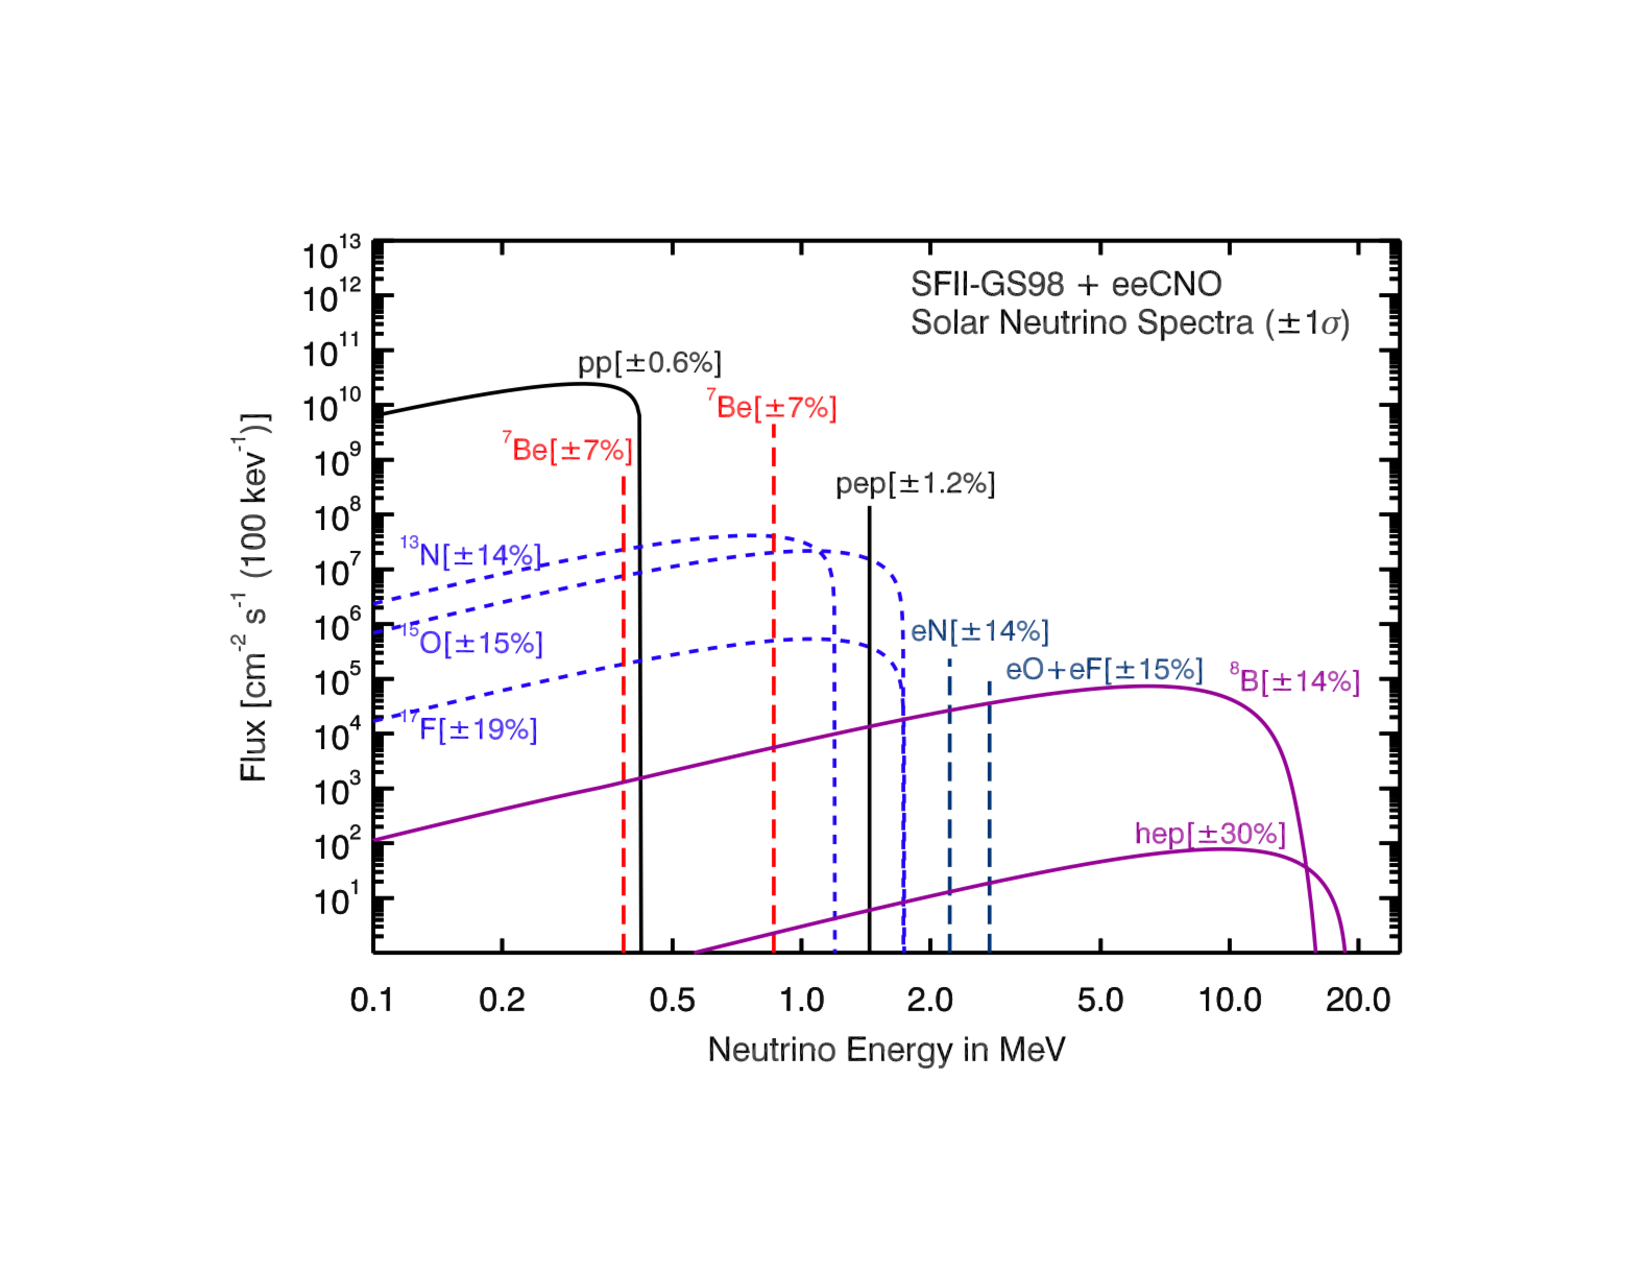
\includegraphics[width=0.7\linewidth]{tex/2-neutrinos-images/SolarFlux}
	\caption[Spectrum of solar neutrino fluxes]{Spectrum of solar neutrino fluxes corresponding to the SFII-GS98 standard solar model. Electron capture CNO neutrinos (ecCNO) have been added in addition to standard fluxes. Electron capture fluxes are given in cm$^{-2}$s$^{-1}$. Figure from Ref.~\cite{Serenelli:2016dgz}.}
	\label{fig:solarflux}
\end{figure}

In the late 1960's, about a decade after Cowan and Reines discovered the first neutrino, astrophysicist John Bahcall and physical chemist Raymond Davis designed an experiment to collect and count solar neutrinos, neutrinos emitted by nuclear fusion taking place in the Sun. 
Davis placed a 380 cubic meter tank filled with perchloroethylene (dry-cleaning fluid) 1,478 meters underground in the Homestake Gold Mine in South Dakota. 
Perchloroethylene was chosen because it is rich in chlorine and the tank was placed deep underground to shield the experiment from cosmic rays. 

Davis was looking for the reaction 
\begin{equation}
	\mathrm{\nu _{e}+ ^{37}Cl \rightarrow  ^{37}Ar+e^{-}} 
	\label{eq:ClAr}
\end{equation}
in which a neutrino would enter the tank and transform chlorine into argon. 
Argon is a noble gas, making it easy to chemically separate from a large amount of chlorine-rich solvent.
This allowed Davis to extract and count the argon atoms, essentially counting the number of neutrinos that had been captured.
The chlorine reaction has a threshold of 814 keV, which, according to standard solar models (see Figure~\ref{fig:solarflux}), allowed the Homestake experiment to detect neutrinos created by $^8$Be in the sun (and $^7$Be, \textit{pep}, $^{13}$N, and $^{15}$O at lower rates).

In the end, with the Homestake experiment Davis calculated a rate of solar neutrinos that was one third of the rate predicted by calculations made by Bahcall using the Standard Model \cite{Davis}. 
This discrepancy became known as the solar neutrino problem, and in the following years Bruno Pontecorvo wrote several theoretical papers proposing neutrino oscillation as a solution \cite{Pont1968,Pont1977}.

Several experiments designed to measure the flux of solar neutrinos followed the Homestake Experiment including SAGE \cite{Abdurashitov:1994bc}, GALLEX \cite{Hampel:1998xg}, and GNO \cite{Altmann:2000ft,Bellotti:2001ta}.
All three experiments built detectors based on the reaction $\mathrm{^{71}Ga(\nu,e^{-})^{71}Ge}$ which has a threshold of 233 keV.
This made them sensitive to neutrinos created by \textit{pp} reactions in the Sun, neutrinos that the Homestake experiment was unable to measure.
Even with the different energy threshold, though, all three experiments showed a deficit in neutrino flux compared to Standard Model calculations and the solar neutrino problem persisted.

Further experimental proof of neutrino oscillation came with results from the Super-Kamiokande Experiment. Unlike previous experiments that were only sensitive to electron neutrinos, Super-K detected neutrinos through elastic scattering of electrons - a process sensitive to all neutrino flavors.
Operating a high threshold of 4 MeV they observed pure $^{8}$Be solar neutrinos, a different selection than previous solar neutrino experiments.
With their large mass, good energy resolution, and ability to determine neutrino directionality, Super-K was able to confirm the solar neutrino problem effect with high statistics and place limits on the parameters of oscillation \cite{SuperKOsc}.

The first direct evidence for solar neutrino flavor change came from the Sudbury Neutrino Observatory (SNO) in 2001 \cite{SNO,SNOOsc}. 
The SNO detector was an imaging Cherenkov detector using heavy water.
They were able to observe neutrino flavor change through three different processes: elastic scattering of electrons, the $\nu_e - d$ charged current reaction (CC), and the $\nu_x - d$ neutral current reaction (NC).
The CC reaction has a threshold of -1.4 MeV, allowing SNO to accurately measure the shape of the $^{8}$B neutrino spectrum.
The CC is also only sensitive to $\nu_{e}$, whereas the NC reaction is sensitive to all three active neutrino flavors, allowing SNO to compare measured fluxes from each reaction and ultimately confirm the theory of neutrino oscillation.

Nearly a century after the initial postulation of the neutrino the scientific community has in hand experimental evidence of three neutrino flavors, mathematical models that include these neutrinos in the Standard Model of Particle Physics, and theoretical and experimental proof that neutrinos oscillate and therefore have mass.
These findings, along with developments in technology and techniques, set the stage for current, and future, neutrino experiments to transform their goals from observing anomalies to making precise measurements of the physics behind the anomalies.
The current best-fit values of the 3-neutrino oscillation parameters as found experimentally are shown in Table~\ref{tab:ParamValues}.


\begin{table}
	\centering
	\begin{tabular}{ccc}
		\hline
		\vspace{-0.3cm} \\ 
		\textbf{Parameter} & \textbf{Best-fit} & \textbf{3$\sigma$} \vspace{0.1cm} \\ 
		\hline 
		\vspace{-0.3cm} \\
		$\Delta m^2_{21}$ [10$^{-5}$ eV$^2$] & 7.37 & 6.93 - 7.96 \\ 
		%\hline 
		\vspace{-0.3cm} \\
		$\Delta m^2_{31(23)}$ [10$^{-3}$ eV$^2$] & 2.56 (2.54) & 2.45 - 2.69 (2.42 - 2.66) \\ 
		%\hline 
		\vspace{-0.3cm} \\
		$\sin^2\theta_{12}$  & 0.297 & 0.250 - 0.354 \\ 
		%\hline 
		\vspace{-0.3cm} \\
		$\sin^2\theta_{23}$  & 0.425 (0.589) & 0.381 - 0.615 (0.384 - 0.636) \\ 
		%\hline 
		\vspace{-0.3cm} \\
		$\sin^2\theta_{13}$  & 0.0215 (0.0216) & 0.0190 - 0.0240 (0.0190 - 0.0242) \\ 
		%\hline 
		\vspace{-0.3cm} \\
		$\delta/\pi$ & 1.38 (1.31) & 2$\sigma$: 1.0 - 1.9 (2$\sigma$: 0.92 - 1.88) \\ 
		\hline 
	\end{tabular} 
	\caption[Neutrino Oscillation Parameters]{The current best-fit values and 3$\sigma$ allowed ranges of the 3-neutrino oscillation parameters as determined experimentally \cite{PDG}. The values (values in brackets) correspond to $m_1 < m_2 < m_3 \hspace{0.1cm} (m_3 < m_1 < m_2)$.}
	\label{tab:ParamValues}
\end{table}


